Given a text $T[1,n]$, we want to process it in order to search on-the-fly for $P[1, p]$ and return occurrences of $P$ as a sub-string of $T$.

NB: on-the-fly means that we have the text (or the dictionary) before and that we will execute different queries, and not that we are given text and pattern together.
In that case we just scan.

NB: $P$ is any sequence of symbols (not forced to sequences of bytes).

An important context of usage is Bioinformatics: we search for DNA sequences.

Here too find occurrences means retrieval of positions and counting.
To solve efficiently we define $T[i, n]$ as a text suffix from position $i$ to position $n$:
\begin{figure}[H]
    \centering
    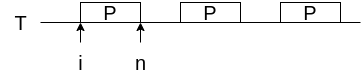
\includegraphics[width=200px]{images/9_Substring/substring_problem.png}
\end{figure}
So we have an occurrence of $P$ in position $i$ if and only if pattern $P$ is prefix of suffix $[i,n]$, so we can reduce the problem to a prefix search!
But we need to manage the space better.

Ex: $T = mississippi\$$, $P=si$: $P$ is a prefix of $T[4,12] = sissippi\$$ and $T[7,12] = sippi\$$ so substring search of $T[1,n]$ is reduced on prefix search on $SUFFIX(T)$ which consists of $n$ suffixes of $T$.

$SUFFIX(T)$ is quadratic: $\sum_{i = 1}^n i = \Theta(n^2)$ so in practical it is not so interesting.

\section{Suffix array}
It's an array which contains all the the prefixes $T[i,n]$ sorted alphabetically:
\begin{table}[H]
    \centering
    \begin{tabular}{c | l}
        $S_A$ & sorted $SUFFIX(T)$ \\
        12 & $\$$ \\
        11 & $i\$$ \\
        8 & $ippi\$$ \\
        5 & $issippi\$$ \\
        2 & $ississippi\$$ \\
        1 & $mississippi\$$ \\
        10 & $pi\$$ \\
        9 & $ppi\$$ \\
        7 & $sippi\$$ \\
        4 & $sissippi\$$ \\
        6 & $ssippi\$$ \\
        3 & $ssissippi\$$ \\
    \end{tabular}
\end{table}
Of course storing sorted $SUFFIX(T)$ is quadratic but we can just store the $S_A$ and $T$ and use $S_A$ as indirection to $T$.

So suffix in position $j$ is $T[S_A[j], n]$, then $S_A$ has size $\Theta(n log_2 n)$ bits and $T$ is $\Theta(n log_2 \sigma)$ bits (using $\sigma$ as alphabet).

Assuming we have a DNA sequence, then we have $\Sigma = \{A, C, G, T\}, \sigma=4$, so $T = 2n$ bits and $S_A = n log_2 n$ bits.
Human genomes is $\approx 2^{30}$ bases, so $n = 2^30$ (1GB) so $S_A$ is $2^{30} log_2 2^{30} = 30 \cdot 2^{30}$ (30GB).

To search we execute a binary search using $S_A$ as index to jump to the text, of course we always search for $P\$$ and $P\#$ to determine the range!

So in the worst case substring search costs $O(p log_2 n)$ time.

NB: for each jump in $S_A$ we will have cache miss because $S_A$ are just indices to $T$.
the count can be gathered just in $log_2 n$ jumps but retrieval needs scan in $S_A$ so it's $O(occ)$ and $O(\frac{occ}{B})$ I/Os, if in the end we would like to retrieve the result sorted we'll have: $O(occ \cdot log_2 occ)$.

NB: in comparison model we can achieve substring search in $O(p + log_2 n)$

\section{Building suffix array}
A non-optimal approach (but elegant) is:
\begin{verbatim}
    SA_build(char *T, int n, char **SA){
        for i = 0; i < n ; i++:
            SA[i] = T+i;
        qsort(SA, n, sizeof(char*), suffix_cmp);
    }

    suffix_cmp(char** p, char** q){
        retur strcmp(*p, *q);
    }
\end{verbatim}
(It's hermetic code).

It's a cubic algorithm but if quicksort on average is $O(n \cdot n log_2 n) = O(n^2 \cdot log_2 n)$, which is still quadratic, not taking into account the cache misses for string comparison.

In the worst case building costs:
$$
    \left( \frac{n}{B} \right) \cdot n log_2 n
$$
I/Os, $n^2 \cdot log_2 n$ time and $n \cdot log_2 n$ extra bits of storage.

NB: there is also a version of this problem which uses prefix tree which uses a trie.

\section{Longest common prefix}
\begin{table}[H]
    \centering
    \begin{tabular}{c | c | l}
        $LCP$ & $S_A$ & sorted $SUFFIX(T)$ \\
        0 & 12 & $\$$ \\
        0 & 11 & $i\$$ \\
        1 & 8 & $ippi\$$ \\
        1 & 5 & $issippi\$$ \\
        4 & 2 & $ississippi\$$ \\
        0 & 1 & $mississippi\$$ \\
        0 & 10 & $pi\$$ \\
        1 & 9 & $ppi\$$ \\
        2 & 7 & $sippi\$$ \\
        1 & 4 & $sissippi\$$ \\
        3 & 6 & $ssippi\$$ \\
         & 3 & $ssissippi\$$ \\
    \end{tabular}
\end{table}
$LCP[i]$ is the length of the longest common prefix between $SA[i]$ and $SA[i+1]$, so it is $LCP[0, n-1]$ and in the worst case can be computed in $O(n^2)$.

It's useful for queries like:
\begin{itemize}
    \item Does it exists a substring of $T$ that repeats (so $\geq 2$) and has length $L$?
    Can be solved using brute-force in $O(n (nL)) = O(n^2)$ but using LCP array we just need to scan for a value $\geq L$ and if there is at least one we return $yes$, otherwise $no$.
    It's a scan over LCP so it is $O(n)$ time and $O\left( \frac{n}{B} \right)$ I/Os.

    \item Find the longest repeated substring.
    Using LCP we just need to find max in LCP which is a scan so $O(n)$ time and $O\left( \frac{n}{B} \right)$.

    \item Check whether exists a substring of length at least $L$ that repeats at least $c$ times.
    Using LCP we look in the array at for at least $L$ and count how many successives are at least $L$, if count is at least $c-1$ we say $yes$, otherwise $no$.
    Basically we are looking for a subarray $LCP[i, i+c-q]$ s.t. each elements $\geq L$.
\end{itemize}




